\chapter{Bosón $W^{\prime}$}\label{Ch:W-prime}
La gran mayoría de los modelos con Física Más Allá de ME (BSM, por sus siglas en ingles) predicen  partículas adicionales al ME. El interés principal en este trabajo consiste en adicionar un bosón vectorial cargado y pesado, generalmente denotado como $W^{\prime}$, con carga $\pm 1$ y espín $1$. En general, dichos modelos también predicen un bosón vectorial neutral, denotado como $Z^{\prime}$. 

Para generar un nuevo bosón vectorial cargado, algunos modelos adicionan dimensión extras a las cuatro dimensiones conocidas. Debido a que estas dimensiones están compactificadas, no es posible verlas a escalas de bajas energía.  Debido a la compactificación de dichas dimensiones, se crean los llamados modos de Kaluza-Klein, que son excitaciones de las partículas del ME en las dimensiones extra. Esto puede predecir excitaciones del  bosón $W$, generando un $W^{\prime}$~\cite{Chen:2009gz, Kong:2010xk}.

Otros modelos proponen una simetría izquierda-derecha, adicionando al grupo mediador del ME un grupo $SU (2)_R$. Después del rompimiento espontaneo de la simetría de este grupo se generan bosones gauge adicionales, tales como, un bosón $W^{\prime}$ y un bosón $Z^{\prime}$~\cite{Boucenna:2016wpr}. Un modelo de referencia que proporciona un $W^{\prime}$ genérico, es el Modelo Estándar Secuencial (MES)~\cite{Altarelli:1989ff}, el cual supone que existe una copia de los bosones $W$ y $Z$ del ME, con masas más grandes ($Z^{\prime}$ y $W^{\prime}$). Los acoples de estos nuevos bosones son diferentes a los bosones del ME.

El Lagrangiano invariante de Lorentz más general posible que describe el acoplamiento de un $W^{\prime}$ a los fermiones del ME, se puede escribir como:
\begin{align}\label{Eq:Lag}
\mathcal{L} = \frac{g}{\sqrt{2}} (Y^{L}_{f_i f^{\prime}_j} W^{\prime}_{\mu} \bar{f}^{i} \gamma^{\mu} P_L f^{j} + Y^{R}_{f_i f^{\prime}_j} W^{\prime}_{\mu} \bar{f}^{i} \gamma^{\mu} P_R f^{j} ) + \text{h.c.}\,,
\end{align}
donde $P_{R,L} = (1 \pm \gamma_5)/2$ es el proyector derecho e izquierdo respectivamente, $g$ es la constante de acople de $SU(2)_L$ del ME, y las $Y^{R,L}_{f_i f^{\prime}_j}$ son los acoples, los cuales son diferentes para cada fermión, ya sea quark o leptón. Para el caso del bosón $W$ del ME, debido a que este solo se acopla a las corrientes izquierdas, tenemos $Y^{R} = 0$, y $Y^{L}$ serían matrices identidad o las respectivas matrices de Cabibbo-Kobayashi-Maskawa (CKM), para leptones y quarks, respectivamente.

Debido a que los acoples del $W^{\prime}$ pueden ser diferentes a los acoples del $W$ del ME, el branching y el ancho de decaimiento  pueden modificarse con respecto al valor del ME. Además, si el $W^{\prime}$ es más pesado que el quark top y el bottom, el decaimiento $W^{\prime} \to t b$ es permitido. Igualmente, los decaimientos de $WZ$ deberían ser tomados en cuenta, pero debido a que estos dependen del modelo, se asume que estos acoples están suprimidos. El ancho total de decaimiento del $W^{\prime}$ sería dividido en tres partes, las cuales dependen del producto de estados finales
%
\begin{align}\label{Eq:Ancho}
\Gamma_{tot} (W^{\prime}) = \sum_{q} \Gamma(W^{\prime} \to t \bar{q}) + \sum_{q q^{\prime}}\Gamma(W^{\prime} \to q \bar{q}^{\prime}) + \sum_{\ell} \Gamma(W^{\prime} \to \ell \bar{\nu_{\ell}})\,,
\end{align}
%
donde $q = u, d, c, s, b$, $\ell = e, \mu, \tau$. Ya que para efectos prácticos el único quark que se considera masivo es el top, por lo que su masa tendrá una contribución en el ancho de decaimiento del $W^{\prime}$. Los anchos de decaimiento para los miembros derechos de la ecuación \eqref{Eq:Ancho} están dados por:
%
\begin{align}
\Gamma(W^{\prime} \to t \bar{q}) =& \frac{|Y_{tq}|^2 g^2}{16 \pi} M_{W^{\prime}}\left( 1 - \frac{M_{t}^2}{M_{W^{\prime}}^2} \right)\left( 1 + \frac{M_{t}^2}{2M_{W^{\prime}}^2} \right)\,, \\
\Gamma(W^{\prime} \to q \bar{q}^{\prime}) =& \frac{|Y_{q q^{\prime}}|^2 g^2}{16 \pi} M_{W^{\prime}}\,, \\
\Gamma(W^{\prime} \to \ell_L \bar{\nu}_{\ell}) =& \frac{|Y_{\ell \bar{\nu}_{\ell}}|^2 g^2}{48 \pi} M_{W^{\prime}}\,,
\end{align}
%
donde $M_{t}$ es la masa del quark top, y se asume que $g^2 = 8M_{W}G_F / \sqrt{2}$ como en el ME. Es de anotar que los anchos de decaimiento del $W^{\prime}$ tienen la misma forma que los del $W$ de ME. La diferencia en los decaimientos está en que $V_{q q^{\prime}}$ se ha reemplazado por $Y_{q q^{\prime}}$, donde $V_{q q^{\prime}}$ son las entradas de la matriz $V_{\text{CKM}}$. El ancho total de decaimiento para el bosón $W^{\prime}$ es:
%
\begin{align}
\Gamma_{\text{tot}}(W^{\prime}) =& \frac{g^2}{16 \pi}\left[\sum_{q}|Y_{tq}|^2 \left( 1 - \frac{M_{t}^2}{M_{W^{\prime}}^2} \right)\left( 1 + \frac{M_{t}^2}{2M_{W^{\prime}}^2} \right) + \sum_{q q^{\prime}} |Y_{q q^{\prime}}|^2 + \sum_{\ell} \frac{|Y_{\ell \bar{\nu}_{\ell}}|^2}{3}\right] M_{W^{\prime}}\,.
\end{align}
%
Comparando con el ancho de decaimiento del bosón $W$ del ME, se tiene una relación entre estos que está dado por la siguiente ecuación:
%
\begin{align*}
\frac{\Gamma_{\text{tot}}(W^{\prime})}{\Gamma_{\text{tot}}(W)}  =& \frac{4}{3} \frac{M_{W^{\prime}}}{M_{W}}\left[\sum_{q}|Y_{tq}|^2 \left( 1 - \frac{M_{t}^2}{M_{W^{\prime}}^2} \right)\left( 1 + \frac{M_{t}^2}{2M_{W^{\prime}}^2} \right) + \sum_{q q^{\prime}}|Y_{q q^{\prime}}|^2 + \sum_{\ell} \frac{|Y_{\ell \bar{\nu}_{\ell}}|^2}{3}\right]\,.
\end{align*}
%
Si se asume que $M_{W^{\prime}} \gg M_{t}$, el branching adquiere la siguiente forma:
%
\begin{align}\label{Eq:Branching}
B(W^{\prime} \to \bar{f} f^{\prime}) = \frac{C_{f f^{\prime}}|Y_{f f^{\prime}}|^2}{ \sum_{f_1 f_1^{\prime}} C_{f_1 f_1^{\prime}} |Y_{f_1 f_1^{\prime}}|^2 }\,,
\end{align}
%
donde $C_{f f^{\prime}}$ hace referencia al factor de color de los fermiones, el cual es $1$ para leptones y $3$ para quarks. 

\section{No niversalidad del $W^{\prime}$}\label{Sec:NoUL}

La Universalidad Leptónica(UL) en el ME se debe a que las tres familias poseen igual hipercarga débil. Además, ésta podría surgir accidentalmente en el ME a bajas energías; lo que implicaría que las anomalías de la universalidad leptónica observadas podrían deberse a que el ME sería un modelo efectivo hasta la escala de TeV.

Sin embargo, no es necesario abandonar la idea de UL para el bosón $W$, debido a que es posible dar explicación a las anomalías observadas, considerando que estas están asociadas con física BSM. Se han propuesto varios modelos teóricos que dan explicación a las anomalías. Dado que, tanto las corrientes débiles neutras, como las corrientes débiles cargadas presentan dichas anomalías, un modelo que da explicación a éstas es el de leptoquarks (LQ)~\cite{Sakaki:2013bfa}. 

Otros modelos que dan explicación a estas anomalías son conocidos como modelos no universales. En estos modelos, se adicionan bosones gauge que se acoplan de forma distinta a las familias de quarks y leptones. La explicación más natural para las anomalías asociadas a corrientes débiles neutras, es la existencia de un nuevo bosón débil neutro, llamado Z prima ($Z^{\prime}$), el cual se acopla de forma diferente a las familias de leptones. Este nuevo bośon puede ser generado a partir de adicionar una  nueva simetría $U(1)$ al ME~\cite{Dalchenko:2017shg}. Ahora, la explicación más natural para las anomalías asociadas a corrientes débiles cargadas, es la existencia de nuevos bosones débiles cargados, llamados $W^{\pm}$ primas ($W^{\prime \pm}$), los cuales se acoplan de forma diferente a las familias de leptones y quarks. Estos nuevos bosones pueden ser generados a partir de adicionar una nueva simetría no Abeliana $SU(2)$ al ME. Es de notar, que es posible incorporar la primera solución a la segunda, en analogía con la simetría $SU(2)$ electrodébil del ME~\cite{Boucenna:2016wpr} donde coexisten el $W$ y el $Z$. 
En dicho modelo también se muestra un mecanismos que permite caracterizar la no universalidad del bosón $W^{\prime}$. Como resultado se obtiene que el $W^{\prime}$ no se acopla a la primera familia. Además, la interacción con la segunda y tercera generación es diferente en general.

Debido a que el interes de este trabajo es poder dar una explicación a las anomalías en $R(D^{(*)})$, tenemos que el decaimiento del mesón $B$ en el ME va a estar suprimido por la $V_{cb}$ de la CKM, como se muestra en la fig.~\ref{Fig:BW_decay}. Por lo tanto es necesario introducir una nueva contribución de las corrientes cargadas, para poder dar explicación a las anomalías. Esta nueva corriente carga se genera apartir de un $W^{\prime}$ no universal.  Las contribuciones debidas al $W^{\prime}$ en $R(D^{(*)})$ se genera por el decaimiento del quark $b$ a un quark $c$ y un bosón $W^{\prime}$, donde a la vez, el $W^{\prime}$ decae a un $\tau$ y a un $\nu$(ver fig.~\ref{Fig:BWp_decay}). Una explicación más detallada de éste modelo se da en el siguiente capítulo.

%
\begin{figure}
\centering
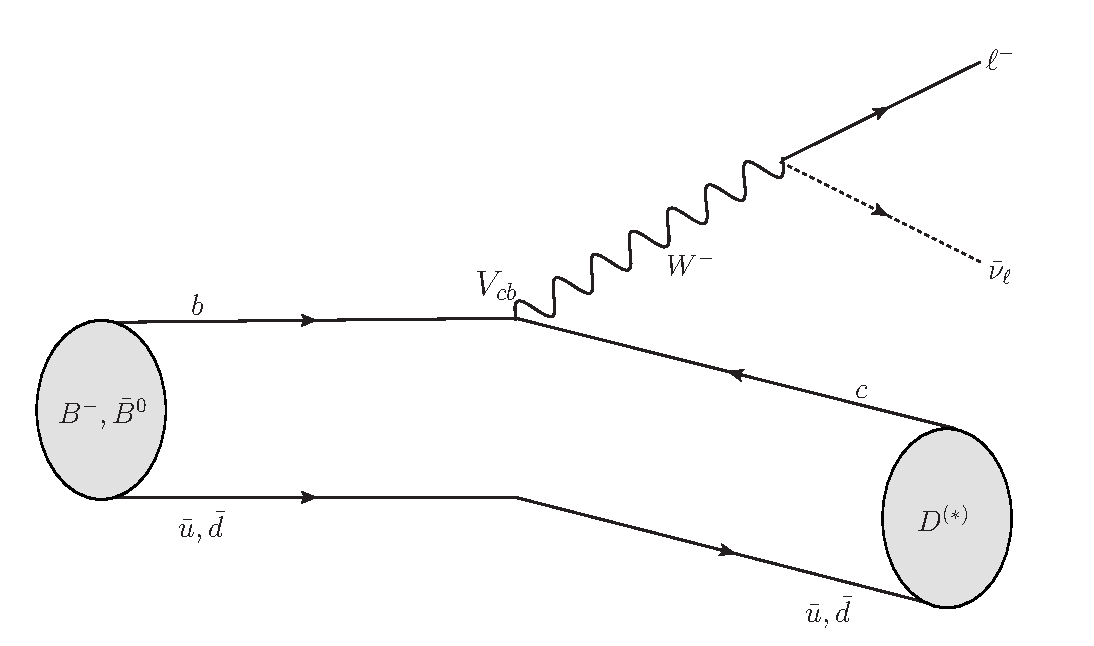
\includegraphics[scale=0.6]{figures/BW_decay}
\caption{Decaimiento en el ME de los mesones $B^{-}, \bar{B}^{0} \to D^{(*)} + \ell^{-} + \bar{\nu}_{\ell}$.}
\label{Fig:BW_decay}
\end{figure}
%

%
\begin{figure}
\centering
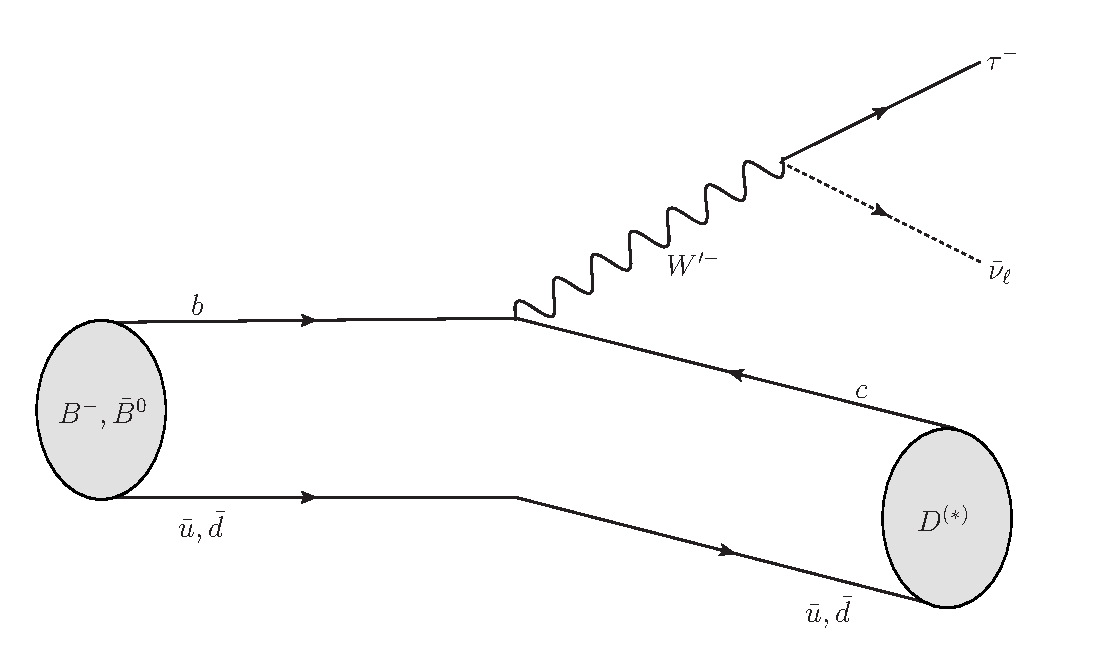
\includegraphics[scale=0.6]{figures/BWp_decay}
\caption{Contribución del $W^{\prime}$ al decaimiento de los mesones $B^{-}, \bar{B}^{0} \to D^{(*)} + \tau^{-} + \bar{\nu}_{\ell}$.}
\label{Fig:BWp_decay}
\end{figure}
%